\documentclass[11pt]{article}
\usepackage[letterpaper,margin=0.85in]{geometry}
\usepackage[T1]{fontenc}
\usepackage{lmodern,amsmath,amssymb,bm,graphicx,booktabs,microtype,longtable}
\usepackage[colorlinks=true,allcolors=blue]{hyperref}
\usepackage[font=small,labelfont=bf]{caption}
\setlength{\emergencystretch}{2em}
\renewcommand{\topfraction}{0.92}
\renewcommand{\textfraction}{0.05}
\renewcommand{\floatpagefraction}{0.65}
\newcommand{\norm}[1]{\left\lVert#1\right\rVert}
\newcommand{\dd}{\mathrm{d}}
\renewcommand{\thesection}{S\arabic{section}}
\renewcommand{\theequation}{S\arabic{equation}}
\renewcommand{\thefigure}{S\arabic{figure}}
\renewcommand{\thetable}{S\arabic{table}}
\newcommand{\RvSingSafeOne}{1410}
\newcommand{\RvSingCertifiedOne}{469}
\newcommand{\RvSingSafeFive}{1942}
\newcommand{\RvSingCertifiedFive}{1105}
\newcommand{\RvSingSafeTen}{2201}
\newcommand{\RvSingCertifiedTen}{1447}
\newcommand{\RvSingSafeTwenty}{2468}
\newcommand{\RvSingCertifiedTwenty}{1957}
\newcommand{\RvAdjCertifiedOne}{497}
\newcommand{\RvAdjCertifiedFive}{1140}
\newcommand{\RvAdjCertifiedTen}{1509}
\newcommand{\RvAdjCertifiedTwenty}{1988}
\newcommand{\RvGaugeError}{8.69\times10^{-16}}

\hypersetup{pdftitle={Supplement: When Can Hall-Silent Valleys Be Neglected in Anomalous-Velocity Nonlinear Hall Transport?},pdfauthor={}}
\title{Supplemental Material\\\large When Can Hall-Silent Valleys Be Neglected in\\Anomalous-Velocity Nonlinear Hall Transport?}
\author{}\date{}
\begin{document}\maketitle
\section{Bands, symmetry and occupied contours}
The Hamiltonian, fixed parameters and momentum centers are specified in the main text. With $\mathcal T=i\sigma_y\mathcal K$, time reversal relates $(s,\bm q)$ to $(-s,-\bm q)$. The mirror internal action $\sigma_x$ relates $(s,q_x,q_y)$ to $(-s,-q_x,q_y)$. Direct substitution transforms each Pauli term and the tilt correctly. The term $s m_r\sigma_z$ respects both operations, so neither protects $m_P=0$. Velocities and Berry curvature are odd under time reversal. Under the mirror $v_x$ and $\Omega_z$ reverse while $v_y$ does not. The geometric $x$ dipole is allowed; the equilibrium Hall integral, $y$ dipole and linear transverse mixing vanish. A constant passive rotation about $\sigma_x$ preserves this symmetry structure.

Let $\delta=\mu-E$. The conduction contour solves
\begin{equation}
\delta=s t q\cos\theta+\sqrt{m^2+v^2q^2}.
\end{equation}
If $v>0$, $|t|<v$ and $\delta>|m|$, its positive radial root is
\begin{equation}
q_F(\theta)=\frac{-\delta st\cos\theta+
\sqrt{v^2(\delta^2-m^2)+m^2t^2\cos^2\theta}}
{v^2-t^2\cos^2\theta}.\label{eq:root}
\end{equation}
The denominator is positive. The squared difference of the square-root term and $|\delta t\cos\theta|$ equals $(v^2-t^2\cos^2\theta)(\delta^2-m^2)>0$. Thus the numerator is positive; substitution into the unsquared equation fixes the branch. The energy along a ray starts below $\mu$, is convex and grows at infinity, giving one positive crossing. Type-I tilt alone is insufficient: for $|m|\sqrt{1-t^2/v^2}<\delta<|m|$, an occupied displaced pocket can have zero or two crossings along a ray. Such pockets require a different quadrature. Equality $\delta=|m|$ does not give strictly positive radii.

The active margin is $1.8-1=0.8$; the smallest passive margin is $0.4-0.1=0.3$. The node of the massless band is outside its conducting contour. Contour validity is enforced during construction and tested independently. Both signs of an invalid mass are rejected in tests. The contour measure and trapezoidal weights are
\begin{equation}
\int\frac{\dd^2q}{(2\pi)^2}\delta(\varepsilon-\mu)X
=\int_0^{2\pi}\frac{q_F\dd\theta}{(2\pi)^2|\partial_q\varepsilon|}X,
\qquad w_i=\frac{q_F}{2\pi N|\partial_q\varepsilon|}.
\end{equation}
The quadratic construction and numerical eigenspinors are checked against the independent root-finding/full-spectral implementation. Berry curvature is independently checked from Hamiltonian derivatives and interband matrix elements, including rotated massive passive states.

\section{Microscopic disorder and basis covariance}
The envelope Hilbert space is sector $\otimes$ partner $\otimes$ internal space. Define
\begin{equation}
T_A=P_A\otimes J,\quad T_P=P_P\otimes J,\quad T_X=\tau_x\otimes J,
\qquad V(\bm r)=\sum_{a=A,P,X}u_a(\bm r)T_a\otimes I,
\end{equation}
where $J_{ss'}=1$. The real fields are independent, zero-mean and Gaussian, with
\begin{equation}
\langle u_a(\bm Q)u_b(\bm Q')\rangle
=(2\pi)^2\delta_{ab}\delta(\bm Q+\bm Q')c_aF_\xi(Q^2),
\quad c_A=c_P=c_0,\quad c_X=\eta c_0.\label{eq:covariance}
\end{equation}
Both $F_\xi(Q^2)=e^{-\xi^2Q^2}$ and $(1+\xi^2Q^2)^{-1}$ are nonnegative spectral covariances. A common finite momentum domain is understood for this continuum disorder model. Diagonal-sector potentials model orbital-energy disorder; the off-diagonal term models random intersector hybridization. These are physically different disorder components. Their independent variances allow a nonnegative control $\eta$, rather than a signed hybridization amplitude. Equality of AA and PP variances and partner-independent matrix magnitudes are simplifying assumptions. Correlated fields and non-scalar internal defect matrices would define different ensembles.

Valley projection brings factors $e^{i(\bm K_j-\bm K_i)\cdot\bm r}$, so the field is evaluated at full $\bm k_j-\bm k_i$. The Born golden-rule energy delta function is absorbed into the contour measure. Independent-field averaging removes cross terms, leaving
\begin{equation}
\mathcal W_{ij}=\Gamma_0a_{r_ir_j}F_\xi(|\bm k_i-\bm k_j|^2)|u_i^\dagger u_j|^2,
\quad a_{AA}=a_{PP}=1,\quad a_{AP}=a_{PA}=\eta.
\end{equation}
For common two-component eigenstates, $|u_i^\dagger u_j|^2=(1+\bm n_i\cdot\bm n_j)/2$. The eigenspinor implementation uses numerical spinors; agreement with the original Bloch-vector formula is separately checked. $\Gamma_0$ absorbs $2\pi c_0/\hbar$ and the declared normalization. This construction realizes the assumed rates but does not fit a microscopic material.

For $\mathcal R_A=I$ and $\mathcal R_P=e^{-i\theta_0\sigma_x/2}$, a physical laboratory texture change uses states $\mathcal R_i u_i$ and unchanged disorder $I$. A gauge/control transformation uses $O'_{ij}=\mathcal R_i I \mathcal R_j^\dagger$, giving
\begin{equation}
\langle \mathcal R_i u_i|O'_{ij}|\mathcal R_j u_j\rangle=\langle u_i|u_j\rangle.
\end{equation}
The code explicitly rotates spinors and transforms the operators. Gauge checks compare rates, kinetic matrices and observables; the largest normalized discrepancy is $\RvGaugeError$. Physical rotations alter AP overlaps and need not preserve responses. Constant $\mathcal R_P$ does preserve dispersion and Berry curvature, as checked independently.

Physical rotation controls use $\theta_0=0,\pi/6,\pi/3,\pi/2$, with laboratory disorder kept fixed. At $m_P=0$ and $\theta_0=\pi/3$, the scalar, shape and weak configurations of the main text have omission errors $2.08996$, $0.218612$ and $0.00390882$, respectively. Their direct passive readout remains zero, so these are collision-mediated effects. The shape representative's signed correction reverses relative to the common-basis result: $S=0.190324$ and $T=-0.920875$. The weak case also loses its especially small cancellation residual. The pointwise results, validity flags and gauge controls are supplied in \texttt{internal\_structure\_robustness.csv} and \texttt{gauge\_invariance.csv}.

The two radial kernels likewise need not give identical finite-range responses. At $(\eta,\delta_P,\xi)=(1,1.2,0.05)$, $m_P=0$ and common texture, Gaussian disorder gives $(H,H_0)=(-2.27642,-3.36017)$ and $e_H=0.476075$, whereas Lorentzian disorder gives $(-2.02064,-3.20202)$ and $e_H=0.584661$. The paired kernel table retains both references and distribution-shape changes; contact cases coincide exactly. These controls support the existence of the kinetic omission mechanism without asserting kernel-independent magnitudes or signs. The physical ablation includes both kernels separately when their finite-range rates differ.

\section{Conservation, projection and exact corrections}
The reversible graph Laplacian obeys
\begin{equation}
x^TLx=\frac12\sum_{ij}\mathcal W_{ij}w_iw_j
\left(\frac{x_i}{\sqrt{w_i}}-\frac{x_j}{\sqrt{w_j}}\right)^2\geq0.
\end{equation}
Consequently $L\sqrt w=0$. At zero intersector coupling there are separate active and passive charge modes; at finite coupling only total charge remains conserved. No physical rate is shifted to regularize them.

An orthonormal odd basis pairs each time-reversed node with its negative, reducing the full $4N$ matrix to $2N$. The drive, transverse drive and Hall readout belong to this invariant subspace. Its active and passive blocks each have dimension $N$ and are positive definite in the tested DC domain. The independent solver uses a full eigenbasis pseudoinverse and explicitly checks drive orthogonality to all removed modes. At finite frequency the complex projected operator is symmetric under transpose, so $M^Tz=h_A$ uses the same factorization structure as a direct solve; it is not a Hermitian adjoint equation. Nevertheless $|z^Tf|\leq\norm z\norm f$ is valid for complex vectors.

Substituting $g_P=F^{-1}(b_P-B^Tg_A)$ gives the main Schur expression. Subtracting $A_{\rm ref}g_{A0}=b_A$ then gives $g_A-g_{A0}=-M^{-1}f$ with $f=(\Delta_A-\Sigma_P)g_{A0}+\zeta_P$. Removing only the off-diagonal block while retaining AP outgoing loss is a different reference. For the affine rate family, $B=\eta K_{AP}$ and $\Delta_A=\eta K_{AA}$. Thus
\begin{align}
\zeta_P&=\eta K_{AP}F_0^{-1}b_P+O(\eta^2),\\
\Sigma_P&=\eta^2K_{AP}F_0^{-1}K_{PA}+O(\eta^3),\\
\Delta H&=-\eta h_A^TA_{\rm ref}^{-1}
\left(K_{AA}g_{A0}+K_{AP}F_0^{-1}b_P\right)+O(\eta^2).
\end{align}
Feedback starts at second order, but is not the entire second-order response. The exact finite-coupling split evaluates all three forcing terms through the same final $z$, so they are not separately switched microscopic mechanisms.

\section{Weighted Hall decomposition and decision statistics}
The weighted least-squares scalar is obtained by differentiating $\norm{g_A-\alpha g_{A0}}^2$ with respect to $\alpha^*$. At finite frequency $\alpha$ is complex. On the DC map $S,T$ and their signs are real. Fractions and $C$ are withheld if
\begin{equation}
|S|+|T|\leq10^{-12}\max(|H_0|,\norm{h_A}\norm{g_{A0}}).
\end{equation}
This convention avoids numerical ratios at exact zero correction. Omission decisions instead use the well-conditioned full Hall response and the fixed-budget envelope defined in the main text.

For each tolerance, truly safe means $|H-H_0|/|H|\leq\epsilon$. Certified safe means the sufficient relative bound is no greater than $\epsilon$. Coverage is certified safe divided by truly safe; false-safe means certified but actually unsafe. Finite informativeness is the fraction with $E<|H_0|$, and useful informativeness at a tolerance is the fraction certified safe among all points. The CSV preserves both definitions, all-point and positive-coupling subsets, and safe/unsafe/uncertified-safe counts. Tightness statistics exclude only exact or numerically negligible corrections where bound/error is undefined; these exclusions do not alter classification counts.

\begin{table}[ht]\centering\small
\begin{tabular}{rrrrr}\toprule
Tolerance & Truly safe & Singular certified & Adjoint certified & False-safe\\\midrule
1\% & \RvSingSafeOne & \RvSingCertifiedOne & \RvAdjCertifiedOne & 0\\
5\% & \RvSingSafeFive & \RvSingCertifiedFive & \RvAdjCertifiedFive & 0\\
10\% & \RvSingSafeTen & \RvSingCertifiedTen & \RvAdjCertifiedTen & 0\\
20\% & \RvSingSafeTwenty & \RvSingCertifiedTwenty & \RvAdjCertifiedTwenty & 0\\\bottomrule
\end{tabular}
\caption{Decision counts for 3510 positive-coupling principal-map points. The two sufficient rules each have zero false-safe points. The inexpensive first-order rule instead has 18, 48, 59 and 66 false-safe points at the four tolerances.}
\end{table}

\section{Physical ablation and invariant-subspace diagnostics}
The final hierarchy uses the four columns and order defined in the main text. Two-pass modified Gram--Schmidt returns $U=U_{\rm raw}\mathsf T$. The tables save the full transformation, raw and orthogonalization norms, current and population overlaps, time-reversal parity, physical-mirror expectation and equal-local-angle partner-exchange expectation. The latter is a diagnostic, not an exact symmetry label for the tilted active pair. $U^TU-I$ and $U_{\rm raw}\mathsf T-U$ are checked for every physical configuration.

\begin{table}[ht]\centering\small
\begin{tabular}{llrrrr}\toprule
Case & Model & Hall error (\%) & $\sigma_{xx}$ error (\%) & $Q_A$ error (\%) & Distribution (\%)\\\midrule
Shape & M1 & 2.063 & 40.58 & 7.892 & 68.48\\
Shape & M2 & 3.056 & 40.58 & 13.52 & 68.5\\
Shape & M3 & 3.742e-14 & 1.839e-14 & 3.586e-14 & 1.021e-13\\
Shape & M4 & 3.742e-14 & 1.839e-14 & 3.586e-14 & 1.012e-13\\
Scalar & M1 & 31.92 & 63.22 & 6.142 & 66.85\\
Scalar & M2 & 0.6807 & 62.98 & 53.84 & 67.04\\
Scalar & M3 & 1.897e-13 & 1.383e-14 & 1.764e-13 & 1.031e-13\\
Scalar & M4 & 1.897e-13 & 1.383e-14 & 1.764e-13 & 1.031e-13\\
Matched range & M1 & 14.88 & 64.34 & 13.33 & 76.74\\
Matched range & M2 & 2.515 & 64.31 & 29.69 & 76.79\\
Matched range & M3 & 7.095 & 0.2498 & 6.942 & 4.75\\
Matched range & M4 & 0.01207 & 0.02972 & 0.01221 & 1.406\\
Weak & M1 & 0.01526 & 74.56 & 0.05638 & 98.2\\
Weak & M2 & 0.03231 & 74.56 & 0.03932 & 98.2\\
Weak & M3 & 0.09868 & 0.007634 & 0.09664 & 7.159\\
Weak & M4 & 0.0001479 & 3.677e-06 & 0.0001482 & 0.01535\\
Fixed-budget & M1 & 4.146 & 59.94 & 4.248 & 89.92\\
Fixed-budget & M2 & 8.855 & 59.94 & 0.8816 & 89.92\\
Fixed-budget & M3 & 16.87 & 0.4772 & 16.57 & 10.86\\
Fixed-budget & M4 & 0.01062 & 0.03873 & 0.01152 & 1.894\\
\bottomrule\end{tabular}
\caption{Extended ordered ablation at the five fixed configurations. All errors use the full observable or weighted distribution norm as denominator. Tiny contact errors are roundoff. No monotonic Hall-error ordering is imposed.}\end{table}
\begin{table}[ht]\centering\small
\begin{tabular}{lrrrr}\toprule
Kernel / range & Min. $\rho_{\rm rel}$ & Max. $\rho_{\rm rel}$ & Max. $\rho_{\rm abs}$ & Max. Hall error (\%)\\\midrule
Gaussian / 0.00 & 6.36e-16 & 5.858e-15 & 1.841e-16 & 2.093e-13\\
Gaussian / 0.05 & 0.006476 & 0.03148 & 0.0008126 & 0.01773\\
Gaussian / 0.10 & 0.01512 & 0.06798 & 0.001163 & 0.3575\\
Lorentzian / 0.00 & 6.36e-16 & 5.858e-15 & 1.841e-16 & 2.093e-13\\
Lorentzian / 0.05 & 0.005365 & 0.02286 & 0.0006286 & 0.03517\\
Lorentzian / 0.10 & 0.01099 & 0.04736 & 0.0009113 & 0.07926\\
\bottomrule\end{tabular}
\caption{Invariant residuals and M4 accuracy on the two-kernel grid, restricted to positive coupling. Contact entries coincide because the kernels are identical. Absolute residuals have collision-rate units; relative residuals are dimensionless.}\end{table}
\begin{table}[ht]\centering\small
\begin{tabular}{rrrrrr}\toprule
Tolerance & Safe & Robust & Dependent & Unsafe & Dependent/safe (\%)\\\midrule
1\% & 1500 & 929 & 571 & 2100 & 38.07\\
5\% & 2032 & 1655 & 377 & 1568 & 18.55\\
10\% & 2291 & 2155 & 136 & 1309 & 5.94\\
\bottomrule\end{tabular}
\caption{Supporting all-grid counts, including 90 decoupled controls: denominator 3600; undefined count zero. Dependent means cancellation-dependent under the fixed-budget test. The principal statistics in the main text exclude these controls.}\end{table}


The ablation projects the full operator at every level. Removing passive coordinates from a Galerkin model does not remove their scattering-out losses. Thus these tests differ from deleting the entire passive sector and all its scattering edges. Conductivity convergence follows the positive quadratic functional $b^TL^{-1}b$, while the bilinear functional $h^TL^{-1}b$ need not converge monotonically. The weighted distribution norm also need not decrease monotonically with nested subspaces, unlike the collision-energy norm.

The relative invariant residual uses spectral norms in numerator and denominator; the supplied Frobenius ratio is a separate statistic. The finite-range Hall-error scatter and the rank correlations are descriptive. All correlations exclude contact roundoff and zero coupling. The drive projection miss is nonzero even where the uncoupled active response is exactly retained, because its collision image need not remain in the same space.

For the Galerkin residual $r_b=b-LUx_4$, the exact DC relation is $H-H_4=z^Tr_b$, $Lz=h$. Since $U^Tr_b=0$, only $(I-UU^T)z$ contributes. With $r_h=h-LUK_4^{-1}U^Th$, the rigorous bounds are
\begin{equation}
|H-H_4|\leq\norm{(I-UU^T)z}\norm{r_b}
\leq\norm{r_h}\norm{r_b}/\lambda_{\min}(L).
\end{equation}
The second inequality follows from $z-UK_4^{-1}U^Th=L^{-1}r_h$. The weaker estimate $\norm h\norm{r_b}/\lambda_{\min}$ is also recorded. These bounds require inverse sensitivity or a relaxation scale; $\rho_{\rm rel}$ alone is not sufficient. At frequency, replace the inverse by $(L+i\omega I)^{-1}$ and the minimum eigenvalue by its smallest singular value.

The spectral diagnostic uses an orthonormal eigenbasis of the full collision operator in the time-reversal-odd space. It records each relaxation rate, drive/Hall overlaps, $\norm{v_\nu^TR_{\rm inv}}^2$, omitted-drive overlap, leakage-forcing overlap, residual overlap and signed Hall-error residue. The leakage-power fraction is a Frobenius quantity, not a decomposition of the spectral norm. Modes can contain retained and complementary components; the complement weight is saved. Degenerate rotations leave grouped powers and residues invariant.

\begin{figure}[!htp]\centering
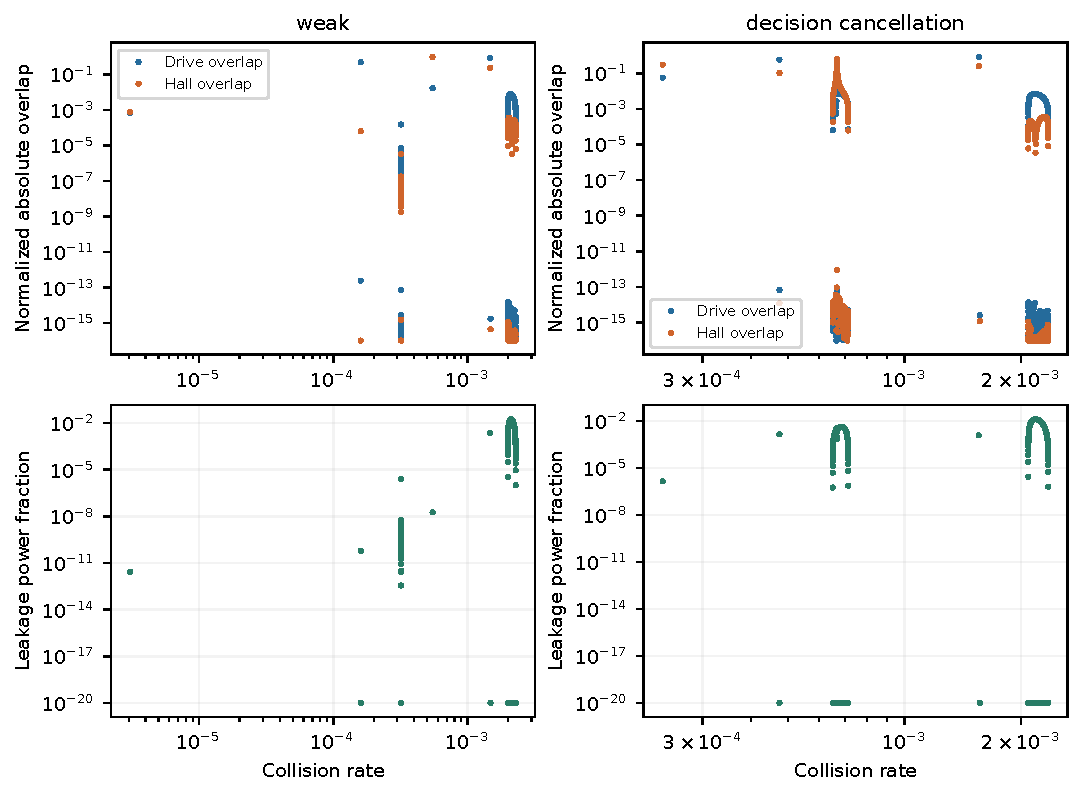
\includegraphics[width=\linewidth]{../figures/supplement/figure_S1_spectral_weights.pdf}
\caption{Drive, Hall and leakage weights in the full collision eigenbasis at the weak and fixed-budget cancellation points. Top: absolute drive and Hall overlaps separately normalized by their Euclidean norms. Bottom: fraction of total Frobenius leakage power. The eigenmodes themselves need not be orthogonal to $U$, although the leakage vector is. These data explain why leakage norm alone does not determine a response error. Numerical display floors are $10^{-16}$ for overlaps and $10^{-20}$ for leakage fractions.}
\end{figure}

\subsection{Physical amplitudes and kernel controls}
The current/population contact space is invariant by the Bloch-moment argument in the main text. No assumption that the Hall vector itself belongs to that space is needed: its projection reads the exact solution in that space. Finite range destroys exact invariance through angular scattering-out rates and nonseparable incoming moments.

The projected active pair has effective coefficients $(a,c,d)$ and source $(p_1,p_2)$, stored with zero-based field names in \nolinkurl{final_reduced_mode_coefficients.csv}. The transmitted passive source's second component is $0.0235031$ and $0.00627817$ for the scalar and shape examples; the residual shape forcing is $-0.00715938$ and $-0.00672774$. Similar forcing can give very different corrections because the stiffness and current-amplitude change differ. The two-kernel ablation uses the fixed grid specified in the main text; all four columns are physically defined, with no fitted response coefficients.

\section{Cancellation envelope and sufficient certificates}
For a fixed component budget $a=|S|+|T|$, maximizing $|D|/|H_0+D|$ over $|D|\leq a$ gives $a/(|H_0|-a)$ when $a<|H_0|$. The maximizer is opposite to $H_0$. The interval or disk reaches a pole when $a\geq|H_0|$, giving an infinite envelope. Two real components with fixed magnitudes instead have four possible signed sums; their discrete maximum is saved separately and can remain finite above this pole threshold. All safe points that are cancellation-dependent under the fixed-budget test at the reported tolerances have $a<|H_0|$ and opposing signs, so these distinctions do not alter the counts.

The envelope describes loss of favorable signs at a fixed budget. It is not a certificate under arbitrary changes in mass, disorder or occupation. A relative decision is withheld if either $|H_0|$ or $|H_0+D|$ is below $10^{-12}\max(|H_0|,a)$; the principal grid has no such point. Vanishing component budget makes fractions and $C$ undefined but gives exact safe omission. At the weak point the same solved response is robust at 1\% and 0.5\% and cancellation-dependent under the fixed-budget test at 0.1\%.

For the exact eliminated problem, the supporting absolute bounds are
\begin{equation}
E_{\rm adj}=\norm z\norm f,\qquad
E_{\rm sing}=\frac{\norm{h_A}\norm f}{s_{\min}(M)},\qquad M^Tz=h_A.
\end{equation}
If $E<|H_0|$, $E/(|H_0|-E)$ bounds the actual relative omission. Both norms discard signed cancellation. Their coverage of truly safe positive-coupling points is 33.26\%, 56.90\%, 65.74\% for the singular bound and 35.25\%, 58.70\%, 68.56\% for the adjoint bound at 1\%, 5\%, 10\%. Neither makes a false-safe decision on the principal grid. The exact identity $\Delta H=-z^Tf$ should be used when $z,f$ are already known; the norm bound does not supply a cheaper exact answer.

An approximate adjoint would satisfy the general residual estimate
\begin{equation}
|\Delta H|\leq|\widetilde z^Tf|+
\frac{\norm{h_A-M^T\widetilde z}\norm f}{s_{\min}(M)}.
\end{equation}
It follows by solving for $z-\widetilde z$ and applying the singular-value bound. No cost or coverage advantage for such an approximation is claimed here: an additional approximate-adjoint study is unnecessary for the physical omission result.

\section{Weak-coupling remainder and sampled intervals}
Set $R_0=[L(0)+i\omega I]^{-1}$, $\mathcal B=\eta R_0K$, and $g_0=R_0b$. Since $L(\eta)+i\omega I=R_0^{-1}(I+\mathcal B)$,
\begin{equation}
g=(I+\mathcal B)^{-1}g_0,\qquad
 g-(I-\mathcal B)g_0=(I+\mathcal B)^{-1}\mathcal B^2g_0.
\end{equation}
Multiplication by $I+\mathcal B$ verifies the exact remainder; no commutation of $R_0$ with $K$ is assumed. If $\rho=\norm{\mathcal B}_2<1$, the Neumann bound gives
\begin{equation}
|H-H_{(1)}|\leq E_N=\frac{\norm h\norm{\mathcal B^2g_0}}{1-\rho}.
\end{equation}
When $E_N<|H_{(1)}|$, a relative error bound is $E_N/(|H_{(1)}|-E_N)$. The spectral radius can establish finite-dimensional convergence but cannot replace the Euclidean norm in this denominator for a nonnormal $\mathcal B$.

At DC, $L_0=L(0)>0$ on the driven space and $K\geq0$. Define $D=L_0^{-1/2}KL_0^{-1/2}$, $\widetilde h=L_0^{-1/2}h$, and $\widetilde b=L_0^{-1/2}b$. Then
\begin{equation}
H=\widetilde h^T(I+\eta D)^{-1}\widetilde b.
\end{equation}
The positive remainder operator has eigenvalues $(\eta\lambda)^2/(1+\eta\lambda)$, increasing for $\lambda\geq0$. With $\rho_{\rm sp}=\eta\lambda_{\max}(D)$,
\begin{equation}
|H-H_{(1)}|\leq E_{\rm energy}=
\norm{\widetilde h}\norm{\widetilde b}\frac{\rho_{\rm sp}^2}{1+\rho_{\rm sp}}.
\end{equation}
This standard positive-matrix bound holds for every $\eta\geq0$, but can be very loose. It is not used at finite frequency. The directional descriptor $\rho_{\rm drive}=\eta\norm{R_0Kg_0}/\norm{g_0}$ is not an operator norm or guaranteed convergence condition.

The comparison uses both radial kernels, $\delta_P=0.4,0.8,1.2$, $\xi=0,0.05,0.10$, and $\omega/\Delta_{\min}=0,0.01$: 36 configurations, each with zero coupling and 31 positive samples between $10^{-5}$ and 1. All 1152 responses use $N=256$ and are compared with $N=128$. Figure~\ref{fig:weak} displays the dependence on several operator descriptors. These plots are descriptive and do not establish a sufficient error criterion. These perturbative controls are distinct from the fixed physical ablation of the main text.

The file \texttt{weak\_coupling\_intervals.csv} reports the last contiguous passing sample, first failure, every passing sampled interval and a sampled-monotonicity flag at 1\%, 5\%, 10\% and 20\%. For example, Gaussian contact disorder at $\delta_P=0.4$, DC, has last-pass/first-fail samples approximately $(0.0681,0.100)$, $(0.147,0.215)$, $(0.316,0.464)$ and $(0.464,0.681)$. These are sampling brackets, not located transition points. Even a monotone sampled sequence does not prove monotonicity between samples. Nonmonotone passing intervals are retained rather than replaced by a single endpoint.

\begin{figure}[!htp]\centering
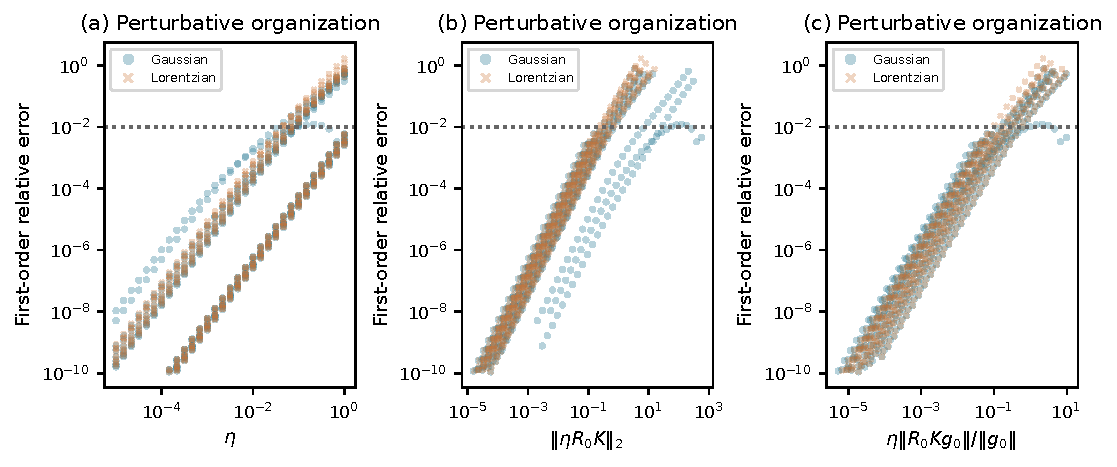
\includegraphics[width=\linewidth]{../figures/supplement/figure_S2_weak_control.pdf}
\caption{First-order response error versus bare coupling, Euclidean operator norm and directional descriptor. Both kernels and all 36 configurations specified in the weak-coupling section are shown for positive coupling and errors above the roundoff floor. These descriptive scatter plots retain larger-error points; their trend is not a certificate. Fixed band parameters and $\Gamma_0=0.01$ match the main text.}\label{fig:weak}
\end{figure}

\section{Cost, memory and asymptotic interpretation}
All five methods start from the same assembled projected matrices, at $(\eta,\delta_P,\xi)=(1,0.8,0.05)$ with $m_P=0$, common basis, Gaussian disorder and $\Gamma_0=0.01$. Wall time uses five repeats after a warm-up and one BLAS thread. Common setup, including geometry, collisions, reference preparation and invariant checks, is timed separately. The full matrix has dimension $2N$; Schur blocks have dimension $N$.

A full Hall solve uses one factorization and one right-hand side. Exact reduction factors $F$ for $N+1$ right-hand sides and then solves $M$. The singular certificate additionally needs an active-reference solve and a smallest-eigenvalue calculation at DC; the adjoint replaces the eigenvalue calculation by a solve with Hall readout. The CSV records the factorization and right-hand-side counts of each implementation. The weak method reuses each reference factor for the zeroth and first correction. No full response is used to construct a certificate value; full responses are calculated separately as ground truth.

Dense elimination costs $O(N_P^3+N_P^2N_A+N_PN_A^2+N_A^3)$ and can generate dense active fill-in. Full dense solution costs $O((N_A+N_P)^3)$. Both have quadratic storage. The saved shared-input bytes and array-workspace estimates exclude LAPACK internals and are not measured peak resident memory. At $N=256$, exact reduction, the singular bound and the adjoint bound cost respectively 1.21, 3.86 and 1.50 times a full solve; at $N=512$ the ratios are 0.89, 3.11 and 1.10. Actual timings and interquartile ranges remain in the CSV; no hardware-independent acceleration claim follows from them. Passive sparsity, reusable factors, analytic inverses or many readouts/drives would change the economics and require separate benchmarks.

\section{Passive mass, direct baseline and continuity}
For the untilted passive band, the positive contour radius is $q_F=\sqrt{\delta_P^2-m_P^2}/v_P$ and the measure is $\delta_P\dd\theta/[(2\pi)^2v_P^2]$. The upper-band two-level curvature is
\begin{equation}
-\frac{\bm d\cdot(\partial_{q_x}\bm d\times\partial_{q_y}\bm d)}{2d^3}
=-\frac{s m_Pv_P^2}{2\delta_P^3}.
\end{equation}
It is constant on each partner contour. Defining $N_s=\sum_{P,s}w_i\ell_i$ therefore gives $H_P=-m_Pv_P^2(N_+-N_-)/(2\delta_P^3)$ exactly. The physical node displacement is reconstructed by lifting the odd-space vector, dividing by $\sqrt w$, and integrating partners separately. The largest discrepancy from direct $h_P^Tg_P$ over the saved grid is below $10^{-11}$.

The exact three-term split in the main text uses $H_P(0,m_P)$ as the direct baseline. The table \texttt{final\_mass\_scaling.csv} explicitly distinguishes direct passive baseline, active coupling and passive coupling, so no subtraction convention is implicit.

The mass sequence is $0,10^{-4},3\times10^{-4},10^{-3},3\times10^{-3},10^{-2},3\times10^{-2},10^{-1}$ at zero and finite coupling for four fixed configurations. Table~\ref{tab:masscontrols} gives the $m_P=0.01$ finite-coupling results. Uncoupled active corrections vanish, as they must.
\begin{table}[ht]\centering\small
\begin{tabular}{lrrrr}\toprule
$(\eta,\delta_P,\xi)$ & $H_P(0,m)$ & $H_A-H_0$ & $H_P(\eta,m)-H_P(0,m)$ & $H_P(\eta,m)$\\\midrule
$(0.001,0.4,0.1)$ & $-2.98783$ & $3.69636\times10^{-5}$ & $-0.211288$ & $-3.19912$\\
$(10,1.2,0)$ & $\simeq0$ & $2.25998$ & $2.08417\times10^{-6}$ & $2.08417\times10^{-6}$\\
$(0.372759,0.4,0)$ & $\simeq0$ & $0.237525$ & $0.000329826$ & $0.000329826$\\
$(1,1.2,0.05)$ & $-0.0675319$ & $1.08693$ & $0.0442284$ & $-0.0233034$\\\bottomrule
\end{tabular}
\caption{Finite passive-mass controls at $m_P=0.01$. The contour-integrated response units and normalization match the main text.}\label{tab:masscontrols}
\end{table}

At fixed valid contours, the collision matrix varies smoothly with mass and has a finite inverse on the driven space at $m_P=0$. Therefore $H_P=m_Ph'_P(0)^Tg_P(0)+O(m_P^2)$. The linear coefficient can be large without being singular. At the weak finite-range point, the massless valley displacements give slopes $-299.528$ and $-321.015$ for $\eta=0$ and $0.001$. At contact disorder the uncoupled polarization vanishes, and the finite-coupling control responses start at order $m_P^2$. These statements hold at fixed occupation and range, not uniformly near a band edge or a vanishing valley relaxation rate.

\begin{figure}[!htp]\centering
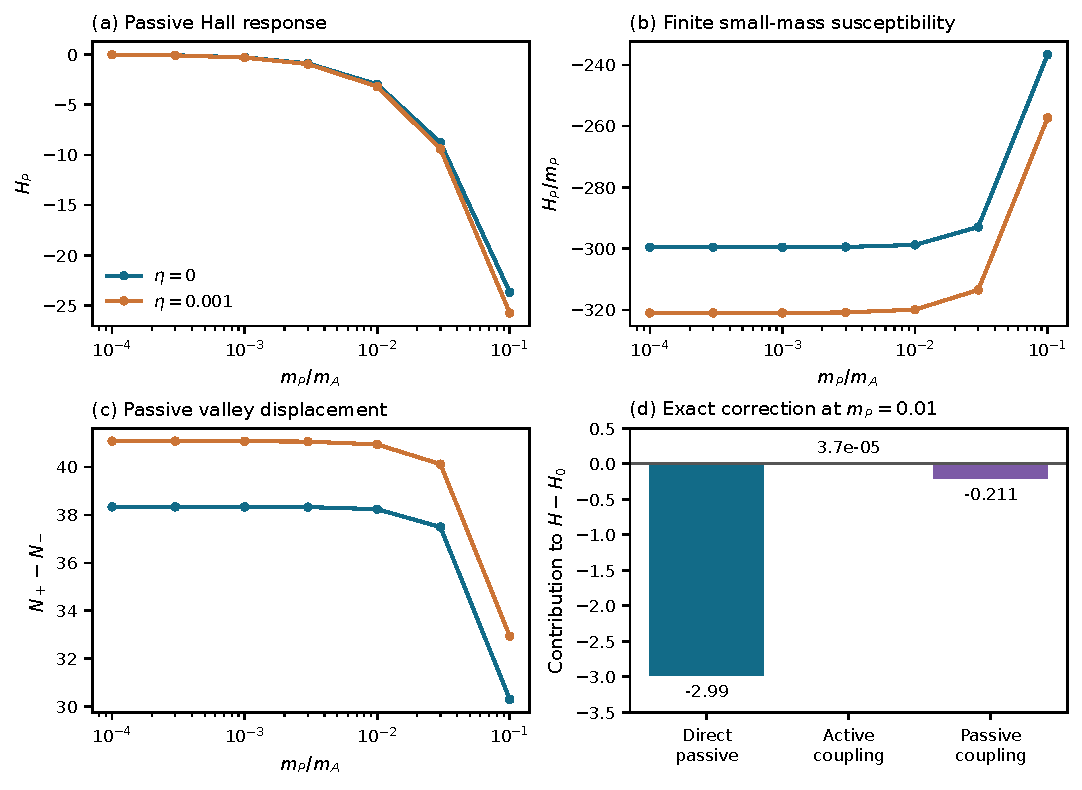
\includegraphics[width=\linewidth]{../figures/supplement/figure_S3_mass.pdf}
\caption{Finite passive-mass control at $\delta_P=0.4$, $\xi=0.1$, Gaussian disorder. The passive Hall response and its ratio to mass approach the finite valley-polarization susceptibility. The signed decomposition at $m_P=0.01$, $\eta=0.001$ separates the direct baseline $H_P(0,m_P)$, active coupling and passive coupling. The large correction is predominantly direct passive readout. The mass dataset and input manifest specify the figure.}
\end{figure}

\section{Response convention and measurement protocols}
Restore $e,\hbar$ with electron charge $-e$, $e>0$. Use $\bm v=\hbar^{-1}\nabla_k\varepsilon$, $\bm{\mathcal A}=i\langle u|\nabla_ku\rangle$, and $E_x(t)=\operatorname{Re}[E_0e^{i\omega t}]$. The force $\hbar\dot{\bm k}=-e\bm E$ and the linearized Boltzmann equation give
\begin{equation}
\delta f^{(1)}=-eD\operatorname{Re}[E_0\ell e^{i\omega t}],\qquad
D=-f'_0\geq0,\qquad (C+i\omega)\ell=v_x.
\end{equation}
The anomalous velocity is $-\dot{\bm k}\times\bm\Omega=(e/\hbar)\bm E\times\bm\Omega$, with $v_y^{\rm an}=-eE_x\Omega_z/\hbar$. Since charge current is $-e\int\bm v f$, the product relevant for $j_y$ has a negative sign. The identity
\begin{equation}
\operatorname{Re}(ae^{i\omega t})\operatorname{Re}(be^{i\omega t})
=\tfrac12\operatorname{Re}(ab^*)+\tfrac12\operatorname{Re}(ab e^{2i\omega t})
\end{equation}
gives
\begin{equation}
j_y^{2\omega}=\chi_{yxx}E_0^2,\qquad
\chi_{yxx}=-\frac{e^3}{2\hbar}H,\qquad H=h^Tg.
\end{equation}
For a momentum-derivative geometric dipole, $D_k=\hbar h^Tb_x$; this accounts for the second $\hbar$ in the usual scalar-lifetime expression. Strict DC combines rectified and second-harmonic pieces and has twice the low-frequency second-harmonic coefficient. Our DC plots mean the $\omega\to0$ second-harmonic limit.

An independent numerical check takes complex $E_0=0.7+0.2i$, constructs the time-dependent occupation shift and vector cross-product anomalous velocity from a coupled solution, and extracts the complex second harmonic from 4096 phases. Three finite frequencies are tested. This validates charge sign, phase and factor $1/2$ independently of the preserved constant-$\tau$ matrix benchmark. The latter tests $(\tau^{-1}+i\omega)g=b_x$ and $H=\tau h^Tb_x/(1+i\omega\tau)$, but does not justify a scalar model for microscopic collisions.

In dimensionless units, $\sigma_{aa}(\nu)=b_a^T(L+i\nu I)^{-1}b_a$. Open circuit requires $0=\sigma_{yy}(2\omega)E_y+\chi(\omega)E_0^2$. For imposed fundamental current $J_0$, $E_0=J_0/\sigma_{xx}(\omega)$. Hence
\begin{equation}
K_E=-\frac{\chi(\omega)}{\sigma_{yy}(2\omega)},\qquad
K_J=-\frac{\chi(\omega)}{\sigma_{yy}(2\omega)\sigma_{xx}(\omega)^2}.
\end{equation}
The denominator contains a complex square. Replacing it by a magnitude square would change the second-harmonic phase. The measurement dataset contains a central coupling sweep and finite-frequency representatives at $\omega/\Delta_{\min}=0.001,0.01$, with real and imaginary parts saved explicitly. Relative errors use the full response in the denominator and can exceed 100\% when the full proxy is small. No complete-channel or material measurement accuracy is inferred.

\section{Numerical validation and supporting controls}
Algebraic validation is separated from discretization, conditioning and physical uncertainty. Independent band, Berry-curvature, conservation, positivity, constant-lifetime, full-pseudoinverse and block-solve tests accompany the code. The compact validation summary records the canonical checks by family. The release validation also recomputes a representative finite-range hierarchy at $N=256$.

Principal, texture, mass and weak-control calculations were compared between $N=128$ and 256; the included convergence summary records counts and worst errors by observable and metric. The three representative cases additionally use $N=48,64,96,128,192,256$, and Fig.~\ref{fig:convergence} plots successive changes. Relative comparisons are used away from zero; tiny signed contributions use a scale-aware absolute criterion. The driven condition number must be below $10^8$, the kinetic residual below $10^{-10}$, and the spectrum positive. These implementation and discretization checks are not physical error bars.

An edge-Laplacian ordering gives a conservative rate envelope. Since $0\leq F_\xi\leq1$ and $a_{rr'}\leq\max(1,\eta)$, compare with contact unit-sector weights. Time-reversed contour spinors have zero total weighted Bloch polarization, also after physical rotations or finite mass. The contact overlap Laplacian is bounded above by $\Gamma_0\mathrm{DOS}_{\rm tot}/2$. Therefore
\begin{equation}
\lambda_{\max}(L)\leq\max(1,\eta)\Gamma_0\mathrm{DOS}_{\rm tot}/2.
\end{equation}
The envelope/interband ratio is below 0.05 throughout the sampled principal and robustness domain. This is a rate-scale check, not a five-percent bound on theoretical error or omitted Hall channels. At DC $L=\Gamma_0\widetilde L$ gives $g,H,\sigma\propto\Gamma_0^{-1}$; dimensionless relative omission and shape fractions do not change. Rate scaling is also checked independently in the automated tests.

\begin{figure}[!htp]\centering
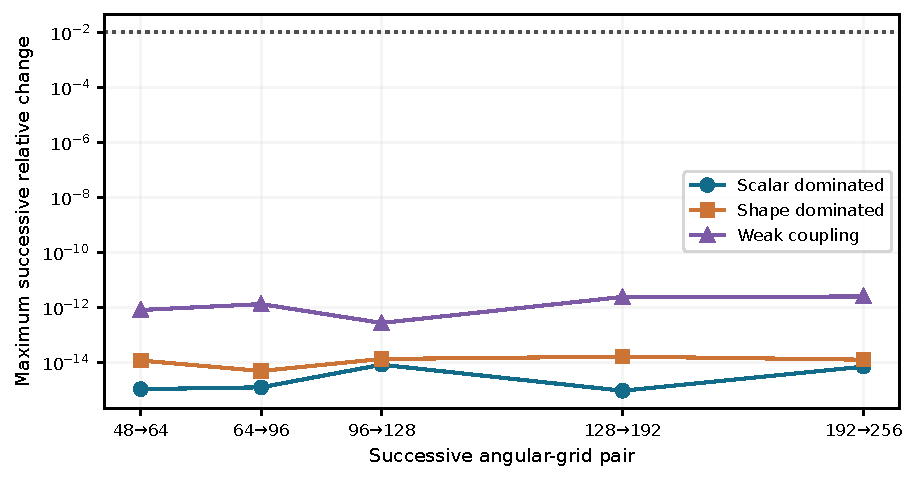
\includegraphics[width=0.88\linewidth]{../figures/supplement/figure_S4_successive_convergence.pdf}
\caption{Successive angular-grid changes for three representative cases: $(\eta,\delta_P,\xi)=(10,1.2,0)$, $(0.372759\ldots,0.4,0)$ and $(0.001,0.4,0.1)$. The maximum over observables using a relative comparison is shown; scale-aware absolute checks are stored separately. Gaussian disorder, $m_P=0$, common basis and $\Gamma_0=0.01$. Values below $10^{-16}$ are displayed at that plotting floor. The dotted line marks the declared one-percent relative threshold.}\label{fig:convergence}
\end{figure}

For an orthonormal driven eigenmode $u_\nu$ of rate $\lambda_\nu$, let $c_\nu=u_\nu^Tb_x$ and $d_\nu=u_\nu^Th$. Then
\begin{equation}
\sigma_{xx}(\omega)=\sum_\nu\frac{c_\nu^2}{\lambda_\nu+i\omega},\qquad
H(\omega)=\sum_\nu\frac{d_\nu c_\nu}{\lambda_\nu+i\omega}.
\end{equation}
Grouping degenerate rates makes residues basis invariant. A common scalar lifetime would require proportional Hall and longitudinal spectral weights in the relevant modes; distinct weights explain frequency-dependent differences. No high-frequency asymptotic or universal scalar-lifetime approximation is assumed.

\section{Scope and reproduction}
The exact Hall difference is an application of standard channel-subtraction and resolvent algebra. Schur elimination, adjoint bounds and goal-oriented error estimation are established tools. The specific contribution is the physical-mode interpretation and tolerance-dependent sector-omission analysis in the stated model. No new mathematical framework or exhaustive priority claim is made.

Side-jump velocities, anomalous distribution terms and skew scattering are not included. The anomalous-velocity nonlinear channel and some omitted terms can share the same disorder scaling; reducing the scattering scale does not isolate a complete response. Physical-model uncertainty therefore remains after numerical convergence: microscopic defects, boundaries, material parameters and additional response channels are not validated by this package.

The data manifest identifies every included table, its source run and checksum. The commands \texttt{make test}, \texttt{make validate}, \texttt{make figures} and \texttt{make paper} run the checks and builds. \texttt{make reproduce-core} reconstructs the principal map, physical ablation, leakage, cancellation and mass controls from explicit settings and compares them with the canonical tables. Supplementary control tables are supplied with source hashes and selected configurations. All figures regenerate without the original working directory or network access after dependencies are installed.
\end{document}
